\documentclass[]{beamer}
\usepackage[english]{babel}
\usepackage[utf8x]{inputenc}
\usepackage{lmodern}
\usepackage[right]{eurosym}
\usepackage{pgfpages}
\usepackage{color}
\usepackage{xcolor}
\usepackage{pgfplotstable}
\usepackage{pgfplots}
\pgfplotsset{width=13cm,compat=1.9}

\usepackage{listings}
\colorlet{mygray}{black!30}
\colorlet{mygreen}{green!60!blue}
\colorlet{mymauve}{red!60!blue}
\colorlet{myyellow}{yellow!50!black}


\lstnewenvironment{C++}{
\lstset{
  backgroundcolor=\color{gray!10},  
  basicstyle=\ttfamily,
  columns=fullflexible,
  breakatwhitespace=false,      
  breaklines=true,                
  captionpos=b,
  belowskip=-2.5em,                    
  commentstyle=\color{DARKGREEN}, 
  extendedchars=true,              
  frame=single,                   
  keepspaces=true,
  showstringspaces=false,             
  keywordstyle=\color{blue},      
  language=c++,                 
  numbers=left,                
  numbersep=5pt,                   
  numberstyle=\tiny\color{blue}, 
  rulecolor=\color{mygray},        
  showspaces=false,               
  showtabs=false,                 
  stepnumber=1,                  
  stringstyle=\color{mymauve},    
  tabsize=3,                      
  title=\lstname                
}}
{}

\lstdefinelanguage{VHDL}{
   morekeywords={
     library,use,all,entity,is,port,in,out,architecture,of,
     begin
   },
   morecomment=[l]--,
   morestring=*[d]{"}
}

\lstnewenvironment{VHI}{
\lstset{
  backgroundcolor=\color{gray!10},  
  basicstyle=\ttfamily,
  columns=fullflexible,
  breakatwhitespace=false,      
  breaklines=true,                
  captionpos=b,
  belowskip=-2.5em,    
  language=VHDL,                 
  commentstyle=\color{DARKGREEN}, 
  extendedchars=true,          
  frame=single,
  showstringspaces=false,                   
  keepspaces=true,
  keywords=[2]{or, and, resize,not,(, ), :, ;},
  keywords=[3]{macro,next, end,else, if, elsif, true, then, is, property, at, t, t_end, false, reset_sequence, assume, prove, freeze, during,[,],t+1,t+2},  
  keywords=[4]{boolean, unsigned, type},          
  keywordstyle=[2]\color{mymauve}, 
  keywordstyle=[3]\color{blue},
  keywordstyle=[4]\color{mygreen},  
  numbers=left,               
  numbersep=5pt,                   
  numberstyle=\tiny\color{blue}, 
  rulecolor=\color{mygray},        
  showspaces=false,               
  showtabs=false,                 
  stepnumber=1,                  
  stringstyle=\color{mymauve},    
  tabsize=3,                      
  title=\lstname                
}}
{}


\usetheme{Frankfurt}

%\beamertemplatenavigationsymbolsempty
%\setbeameroption{show notes on second screen=left}

\title{Multilevel Hardware Generation and Verification}
\subtitle{Presentation of master thesis}
\author{Harald Øvsthus}

\begin{document}
	\begin{frame}[plain]

		\titlepage
	\end{frame}

	\begin{frame}
		\frametitle{Contents of presentation}
		\tableofcontents
	\end{frame}

	\section{Introduction}
	\begin{frame}
		\frametitle{Introduction}
	          \onslide<1->{\textbf{Idea:}}
                  \begin{itemize}
	           \item<1->Generate AMBA-AHB systems at the ESL and RTL
                   \item<1->Generate properties from the ESL, automatically refine them
                  \end{itemize}
                  \onslide<2->{\textbf{Goals:}}
                    \begin{enumerate}
                      \item<2-> Abstraction
                      \item<2-> Soundness
                    \end{enumerate}     
	\end{frame}

       \section{RTL overview}
         \begin{frame}
           \frametitle{RTL overview}
           \begin{columns}
            \column{0.5\textwidth}
             \begin{itemize}
             \item<1-> Reuse open source AHB architecture
             \item<2-> Agents implement the protocol
             \end{itemize}
            \column{0.5\textwidth}
             \centering
             \only<1>{\includegraphics[width=0.7\textwidth]{pics/OS_HW.png}}
             \only<2>{\includegraphics[width=\textwidth]{pics/RTL_overview.png}}
           \end{columns}
         \end{frame}

       \section{ESL overview}
         \begin{frame}
          \frametitle{ESL overview}
          \begin{columns}
           \column{0.5\textwidth}
             \begin{enumerate}
              \item<1-> Master agent PPA
               \begin{itemize}
                \item<1-> Stores and issues request, handles response
                \item<1-> All act in parallel/pipeline
                \item<1-> Lowers abstraction, but necessary
               \end{itemize}
              \item<2-> Bus matrix PPA
                \begin{itemize}
                \item<2-> Includes slave agents
                \item<2-> Pipelined interaction with master agents
                \item<2-> Each stage in pipeline is important state
               \end{itemize}
             \end{enumerate}
           \column{0.5\textwidth}
             \includegraphics[width=\textwidth]{pics/ESL_overview_2.png}
          \end{columns}
         \end{frame}

      \subsection{Port emulation}        

         \begin{frame}
          \frametitle{Port emulation}
          \begin{columns}
           \column{0.5\textwidth}
              \begin{itemize}
               \item<1-> Up to three masters are pipelined
               \item<2-> Requests and two transfer phases are handled concurrently
               \item<3-> Blocking interfaces enable synchronization
               \item<4-> \alert{Only one blocking read/write per time point allowed}
              \end{itemize}
           \column{0.5\textwidth}
             \only<1>{\includegraphics[width=\textwidth]{pics/port_em_1.png}}
             \only<2>{\includegraphics[width=\textwidth]{pics/port_em_2.png}}
             \only<3>{\includegraphics[width=\textwidth]{pics/port_em_3.png}}
             \only<4>{\includegraphics[width=\textwidth]{pics/port_em_4.png}}
          \end{columns}
         \end{frame}

         \begin{frame}
           \frametitle{Port soundness}
         \begin{columns}
           \column{0.5\textwidth}
             \begin{itemize}
               \item<1-> Fixed-priority arbitration is easily mirrored
               \item<2-> No wait statements are called
               \item<3-> Requests are forwarded 
               \item<4-> All threads advance synchronized
             \end{itemize} 
           \column{0.5\textwidth}
             \only<1>{\includegraphics[width=\textwidth]{pics/Soundness0.png}}
             \only<2>{\includegraphics[width=\textwidth]{pics/Soundness1.png}}
             \only<3>{\includegraphics[width=\textwidth]{pics/Soundness2.png}}
             \only<4>{\includegraphics[width=\textwidth]{pics/Soundness3.png}}

          \end{columns}
         \end{frame}

       \subsection{Completeness}
       \begin{frame}
        \frametitle{Completeness}
          \begin{enumerate}
             \item<1-> Master agent completeness
              \begin{itemize}
                \item<1-> All I/O listed in completeness description
                \item<1-> All completeness checks hold, no constraints
                \item<1-> State added as cluster output
              \end{itemize}
             \item<2-> Bus matrix completeness
              \begin{itemize}
                \item<2-> Default master state helps determine bus state
                \item<2-> All I/O listed in completeness description
                \item<2-> All completeness checks hold, no constraints
              \end{itemize}
          \end{enumerate}
       \end{frame}

       \begin{frame}
         \frametitle{Completeness continued}
           \begin{center}
           \includegraphics[width=0.3\textwidth]{pics/port_refine.png}
           \end{center}
           \fontsize{8pt}{12}\selectfont
           \only<1,2>{\textcolor{blue}{macro} Agent\_request\_notify := \textit{hbusreqx} \\\textcolor{blue}{macro} Agent\_request\_sync := \textit{hready \textcolor{red!60!blue}{and} \textit{hgrant}} \\\textcolor{blue}{macro} Bus\_ready\_sync := \textit{hready}\\}
           \only<2>{\textcolor{red}{-----------------\\}}
           \only<2>{\textcolor{blue}{macro} Requests\_sig\_m0 := \textit{hbusreq0} \\ 
                    \textcolor{blue}{macro} Requests\_sig\_m1 = \textit{hbusreq1} \\
                    \textcolor{blue}{macro}  Update\_requests\_notify := \\ \textit{hready0 \textcolor{red!60!blue}{and} hready1 \textcolor{red!60!blue}{or} \\ hready0 \textcolor{red!60!blue}{and} hgrant0 \textcolor{red!60!blue}{or} hready1 \textcolor{red!60!blue}{and} hgrant1}}
       \end{frame}

       \subsection{Simulation}

         \begin{frame}
           \frametitle{Simulation}
           \begin{columns}
             \column{0.5\textwidth}
              \begin{itemize}
               \item<1-> Testbenches modeled equally at ESL and RTL
               \item<2-> Dummies perform write and read operations
               \item<3-> Slave IDs are encoded in data, both directions
               \item<4-> Assertions catch if wrong slave/master is receives payload 
              \end{itemize}
             \column{0.5\textwidth}
             \includegraphics[width=\textwidth]{pics/tb_esl.png}
           \end{columns}
         \end{frame}

        \section{Results}
         \begin{frame}
\frametitle{Simulation Time Comparison}
\begin{itemize}
 \item ESL unaffected by latency and size
 \item ESL is $>$ 10x faster than RTL's best case
\end{itemize}
\begin{center}
\begin{tikzpicture}[scale=0.5]
\begin{axis}[
    title={Simulation time, $10^6$ transactions},
    xlabel={N.o. Slaves},
    ylabel={Time in seconds},
    xmin=1, xmax=15,
    ymin=0, ymax=300,
    xtick={1,5,10,15},
    ytick={7,50,70,100,150,200,250,300},
    legend pos=outer north east,
    ymajorgrids=true,
    grid style=dashed,
]
\only<1->{\addplot[
    color=blue,
    mark=square,
    ]
    coordinates {
    (1,261)(5,266)(10,270)(15,284)

    };
    \addlegendentry{RTL, 1 master}}

\only<1->{\addplot[
    color=blue,
    mark=*,
    ]
    coordinates {
    (1,161)(5,166)(10,180)(15,195)
    };
    \addlegendentry{RTL, 2 masters}}

\only<1->{\addplot[
    color=red,
    mark=*,
    ]
    coordinates {
    (1,77)(5,86)(10,103)(15,125)
    };
    \addlegendentry{RTL, 3 masters}}

\only<2->{\addplot[
    color=black,
    mark=x,
    ]
    coordinates {
   (1,89)(5,96)(10,116)(15,132)
    };
    \addlegendentry{RTL, 5 masters}}

\only<2->{\addplot[
    color=red,
    mark=square,
    ]
    coordinates {
    (1,93)(5,106)(10,128)(15,138)
    };
    \addlegendentry{RTL, 10 masters}}

\only<2->{\addplot[
    color=black,
    mark=square,
    ]
    coordinates {
    (1,105)(5,115)(10,136)(15,143)
    };
    \addlegendentry{RTL, 15 masters}}
    
\only<1->{\addplot[
    color=black,
    mark=*,
    ]
    coordinates {
    (1,7)(5,7)(10,7)(15,7)
    };
    \addlegendentry{ESL, 1-15 masters}}
\end{axis}
\end{tikzpicture}
\end{center}
\end{frame}

\begin{frame}
\frametitle{Properties and Proof times}
\begin{itemize}
 \item Property count only depends on slaves
 \item Proof time dependent on masters and slaves
 \item Vacuous/unreachable properties in 1-2 master systems
\end{itemize}
 \begin{columns}
\column{0.5\textwidth}
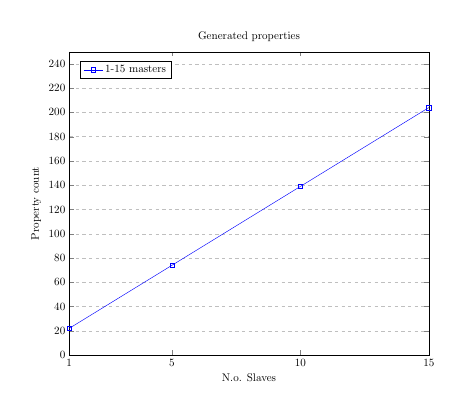
\begin{tikzpicture}[scale=0.4]
\begin{axis}[
    title={Generated properties},
    xlabel={N.o. Slaves},
    ylabel={Property count},
    xmin=1, xmax=15,
    ymin=0, ymax=250,
    xtick={1,5,10,15},
    ytick={0,20,40,60,80,100,120,140, 160, 180, 200, 220, 240},
    legend pos=north west,
    ymajorgrids=true,
    grid style=dashed,
]
\addplot[
    color=blue,
    mark=square,
    ]
    coordinates {
    (1,22)(5,74)(10,139)(15,204)

    };
    \addlegendentry{1-15 masters}


\end{axis}
\end{tikzpicture}
\column{0.5\textwidth}
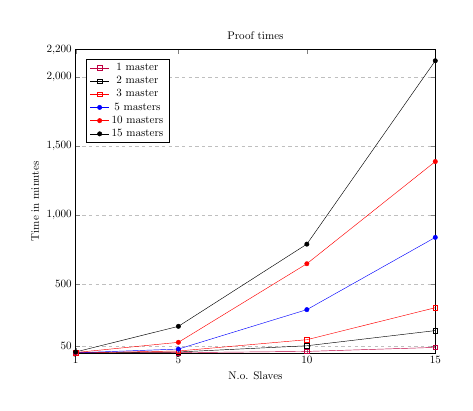
\begin{tikzpicture}[scale=0.4]
\begin{axis}[
    title={Proof times},
    xlabel={N.o. Slaves},
    ylabel={Time in minutes},
    xmin=1, xmax=15,
    ymin=0, ymax=2200,
    xtick={1,5,10,15},
    ytick={50,500, 1000, 1500, 2000, 2200},
    legend pos=north west,
    ymajorgrids=true,
    grid style=dashed,
]
\addplot[
    color=purple,
    mark=square,
    ]
    coordinates {
    (1,1)(5,2)(10,11)(15,40)

    };
    \addlegendentry{1 master}

\addplot[
    color=black,
    mark=square,
    ]
    coordinates {
    (1,1)(5,7)(10,52)(15,162)

    };
    \addlegendentry{2 master}

\addplot[
    color=red,
    mark=square,
    ]
    coordinates {
    (1,1)(5,14)(10,96)(15,328)

    };
    \addlegendentry{3 master}

\addplot[
    color=blue,
    mark=*,
    ]
    coordinates {
   (1,1)(5,28)(10,314)(15,838)
    };
    \addlegendentry{5 masters}

\addplot[
    color=red,
    mark=*,
    ]
    coordinates {
    (1,3)(5,77)(10,647)(15,1388)
    };
    \addlegendentry{10 masters}

\addplot[
    color=black,
    mark=*,
    ]
    coordinates {
    (1,7)(5,193)(10,789)(15,2119)
    };
    \addlegendentry{15 masters}
    
\end{axis}
\end{tikzpicture}

 \end{columns}
\end{frame}


\subsection{Starvation}
 \begin{frame}
  \frametitle{Starvation}
   \begin{columns}
     \column{0.5\textwidth}
       \begin{itemize}
         \item<1-> Fixed-priority is vulnerable to starvation
         \item<2-> How is this time-dependency reflected in an untimed model?
         \item<3-> Time has two meanings at the ESL: 
          \begin{enumerate}
           \item<3-> Simulation time
           \item<3-> Context switches
          \end{enumerate}
         \item<4-> Systems of $>$3 masters are vulnerable 
       \end{itemize}
     \column{0.5\textwidth}
        \only<1>{\includegraphics[width=\textwidth]{pics/starve.png}}
        \only<2>{\includegraphics[width=\textwidth]{pics/starve2.png}}
        \only<3>{\includegraphics[width=\textwidth]{pics/starve3.png}}
        \only<4>{\includegraphics[width=\textwidth]{pics/starve4.png}}
   \end{columns}
 \end{frame}


         \begin{frame}
           \frametitle{Starvation comparison}
          \only<1>{Simplified model, all rates are equal between masters}
          \only<2>{SC\_ZERO\_TIME is measured in context switches}
          \only<3>{Nearly no variation in ESL model}
          \only<4>{Random times reduces probability of grants}
          \only<5>{A monitor is feasible, with two restrictions}
          \begin{columns}
             \column{0.5\textwidth}
\begin{tikzpicture}[scale=0.4]
\begin{axis}[
    title={Master grant delay, RTL},
    xlabel={Master granted},
    ylabel={Clock delay between transfers},
    xmin=1, xmax=15,
    ymin=0, ymax=60,
    xtick={1,2,3,4,5,6,7,8,9,10,11,12,13,14,15},
    ytick={0,2,4,6,8,10,12,14,16,18,20,22,24,26,28,30,32,34,36,38,40,42,44,46,48,50,52,54,56,58,60},
    legend pos=north west,
    ymajorgrids=true,
    grid style=dashed,
]
\only<1,2->{\addplot[
    color=blue,
    mark=square,
    ]
    coordinates {
    (1,0)(2,0)(3,0)(4,0)(5,2)(6,4)(7,6)(8,8)(9,10)(10,12)(11,14)(12,16)(13,18)(14,20)(15,22)

    };
    \addlegendentry{Out of range}}

\only<3->{\addplot[
    color=purple,
    mark=square,
    ]
    coordinates {
    (1,0)(3,0)(5,6)(7,14)(9,22)(11,30)(13,38)(15,46)

    };
    \addlegendentry{write success}}

\only<3->{\addplot[
    color=red,
    mark=*,
    ]
    coordinates {
    (1,0)(2,0)(4,2)(6,10)(8,18)(10,26)(12,34)(14,42)(15,46)

    };
    \addlegendentry{read error}}

\only<3->{\addplot[
    color=black,
    mark=square,
    ]
    coordinates {
    (1,0)(2,0)(3,0)(4,1)(5,4)(6,7)(7,10)(8,13)(9,16)(10,19)(11,22)(12,25)(13,28)(14,31)(15,34)
    };
    \addlegendentry{read success}}

\only<3->{\addplot[
    color=gray,
    mark=square,
    ]
    coordinates {
    (1,0)(2,0)(3,0)(4,3)(5,8)(6,13)(7,18)(8,23)(9,28)(10,33)(11,38)(12,43)(13,48)(14,53)(15,58)

    };
    \addlegendentry{write error}}

\end{axis}
\end{tikzpicture}
             \column{0.5\textwidth}
\begin{tikzpicture}[scale=0.4]
\begin{axis}[
    title={Master grant delay, ESL},
    xlabel={Master granted},
    ylabel={x},
    xmin=1, xmax=15,
    ymin=0, ymax=25,
    xtick={1,2,3,4,5,6,7,8,9,10,11,12,13,14,15},
    ytick={0,2,4,6,8,10,12,14,16,18,20,22,24},
    legend pos=north west,
    ymajorgrids=true,
    grid style=dashed,
]

\only<4->{\addplot[
   color=red,
    mark=square,
    ]
    coordinates {
    (1,0)(2,0)(3,0)(4,2)(5,3)(6,4)(7,5)(8,6)(9,7)(10,9)(11,11)(12,13)(13,14)(14,21)(15,22)

    };
    \addlegendentry{single wait, in range, random, $y=4$}}

\only<4->{\addplot[
   color=blue,
    mark=square,
    ]
    coordinates {
    (1,0)(2,0)(3,0)(4,2)(5,3)(6,4)(7,5)(8,6)(9,7)(10,8)(11,9)(12,11)(13,12)(14,14)(15,16)

    };
    \addlegendentry{single wait, in range, random, $y=2$}}



\only<3->{\addplot[
   color=purple,
    mark=*,
    ]
    coordinates {
    (1,0)(2,0)(3,0)(4,2)(5,3)(7,5)(8,6)(10,8)(12,10)(14,12)(15,13)

    };
    \addlegendentry{single wait, in range, fixed}}


\only<1->{\addplot[ 
  color=black,
    mark=square,
    ]
    coordinates {
    (1,0)(2,0)(3,0)(4,1)(5,3)(6,4)(7,5)(9,7)(11,9)(13,11)(15,13)

    };
    \addlegendentry{single wait, out of range, fixed wait}}

\only<2,5>{\addplot[ 
  color=red,
    mark=*,
    ]
    coordinates {
    (1,0)(2,0)(3,0)(4,2)(5,2)(6,4)(7,4)(8,6)(9,6)(10,8)(11,8)(12,10)(13,10)(14,12)(15,12)

    };
    \addlegendentry{context switch, out of range, SC\_ZERO\_TIME}}


\end{axis}
\end{tikzpicture}
 \end{columns}
 \end{frame}    

\section{Generator}
 \begin{frame}
  \frametitle{Generator}
    \begin{itemize}
      \item<1-> Hardware generator
        \begin{enumerate}
          \item<1-> Reads slave address ranges from customizable file
          \item<1-> Generates ESL and RTL files
          \item<1-> Calls plugin with ESL 
        \end{enumerate}
      \item<2-> DeSCAM plugin
        \begin{enumerate}
          \item<2-> Differentiates between agent and bus matrix
          \item<2-> Creates a refined property set for agent and bus matrix
          \item<2-> Generates completeness descriptions
        \end{enumerate}
    \end{itemize}
 \end{frame}

\section{Burst transfers}
 \begin{frame}
  \frametitle{Concept: Burst transfers}
         \only<1>{\includegraphics[scale=0.5]{pics/burst_esl_stripped.png}}
         \only<2->{\includegraphics[scale=0.5]{pics/burst_esl.png}}
    \begin{itemize}
      \item<1-> Payloads are extended to include burst
      \item<2-> Additional ports are required 
    \end{itemize}  
 \end{frame}

 \begin{frame}[fragile]
   \frametitle{Bursts continued}
 
  \begin{VHI}
payload.htrans = seq | seq | seq | nonseq;
payload.hwdata3 = data3;
payload.hwdata4 = 0;

macro hwdata4_sig := 
if(16-beat burst) then
prev(hwdata,11)
elsif(8-beat burst) then
prev(hwdata,3)
else
resize(0,32)
end if;
end macro;
  \end{VHI}
 \end{frame}

\begin{frame}
 \frametitle{Bursts continued}
 Where do we stand with completeness?
 \begin{itemize}
  \item<1-> Determination requirements
  \item<2-> Duration of transfer
 \end{itemize}
\end{frame}

\section{Final thoughts}

\begin{frame}
 \frametitle{What remains}
 \begin{enumerate}
  \item<1-> Formally verified emulated port
  \item<2-> Monitor for fixed-priority arbitration
  \item<3-> Add burst transactions to the generator
  \item<4-> Add split and retry response types
 \end{enumerate}
\end{frame}

\begin{frame}
 Questions?
\end{frame}

\end{document}
